\documentclass[tikz,border=5mm]{standalone}
\usepackage{amsmath}
\usetikzlibrary{decorations.pathreplacing}

\begin{document}

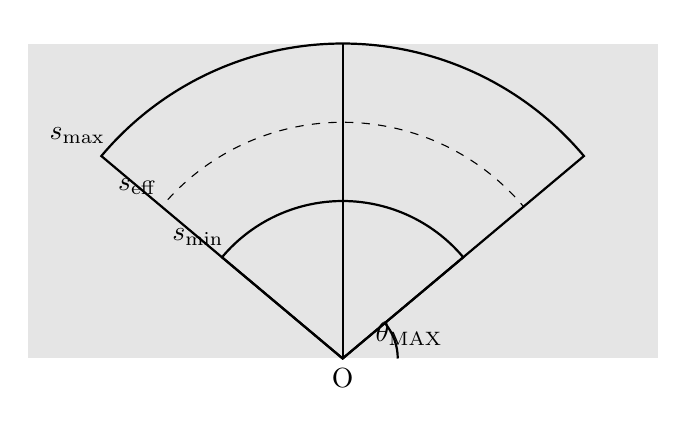
\begin{tikzpicture}

% Background
\fill[gray!20] (-4,0) rectangle (4,4);

% Define distances
\def\smin{2}
\def\smax{4}
\def\seff{3}

% Draw arcs
\draw[thick] (0,0) -- (40:\smin) arc (40:140:\smin) -- cycle;
\draw[thick] (0,0) -- (40:\smax) arc (40:140:\smax) -- cycle;

% Dashed arc for s_eff
\draw[dashed] (0,0) -- (40:\seff) arc (40:140:\seff) -- cycle;

% Draw radial lines
\draw[thick] (0,0) -- (90:\smin);
\draw[thick] (0,0) -- (90:\smax);
\draw[dashed] (0,0) -- (90:\seff);

% Angle mark
\draw[thick] (0:0.7) arc (0:40:0.7);
\node at (20:0.9) {$\theta_{\mathrm{MAX}}$};

% Labels
\node at (140:\smin+0.4) {$s_{\mathrm{min}}$};
\node at (140:\smax+0.4) {$s_{\mathrm{max}}$};
\node at (140:\seff+0.4) {$s_{\mathrm{eff}}$};

% Origin label
\node[below] at (0,0) {O};

% Dotted radial lines for angular opening
\draw[dotted] (0,0) -- (40:\smax);
\draw[dotted] (0,0) -- (140:\smax);

\end{tikzpicture}

\end{document}